% Standalone figure: run make in this directory to build PDF and SVG.
\documentclass[11pt,tikz,border=0pt]{standalone}
\usepackage{fontspec}
\IfFontExistsTF{Helvetica Neue Light}{
  \setsansfont{Helvetica Neue Light}[BoldFont={Helvetica Neue Medium}]
  \newfontfamily\vnmedium{Helvetica Neue Medium}
}{
  \setsansfont{TeX Gyre Heros}
  \newcommand{\vnmedium}{\bfseries}
}
\renewcommand{\familydefault}{\sfdefault}
\usepackage{amsmath,amssymb,mathtools}
\usepackage{unicode-math}
\setmathfont{latinmodern-math.otf}
\usetikzlibrary{arrows.meta,calc,positioning}
\definecolor{vnslideink}{HTML}{333333}
\definecolor{vnslidebody}{HTML}{5E5E5E}
\definecolor{vnaccent}{HTML}{FF644E}
\definecolor{vnslidelink}{HTML}{579ACA}
\pagecolor{white}
\tikzset{
  graphvertex/.style={draw=vnslideink,circle,fill=white,line width=0.7pt,
    minimum size=7mm,inner sep=0pt,font=\small\vnmedium},
  graphedge/.style={draw=vnslidebody,line width=0.8pt},
  grapharrow/.style={draw=vnslidebody,line width=0.8pt,-{Latex[length=2.5mm]}},
  graphaccent/.style={draw=vnaccent,line width=1.2pt,-{Latex[length=2.5mm]}},
}

\begin{document}
\color{vnslidebody}
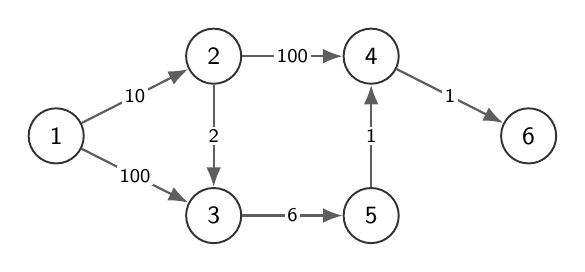
\begin{tikzpicture}[x=1.0cm,y=0.92cm]
        \foreach \n/\x/\y in {1/0/1.4,2/2/2.5,3/2/0.3,4/4/2.5,5/4/0.3,6/6/1.4}
          {\node[graphvertex] (v\n) at (\x,\y) {\n};}
        \foreach \a/\b/\w in {1/2/10,1/3/100,2/3/2,2/4/100,3/5/6,4/6/1,5/4/1}
          {\draw[grapharrow] (v\a)--node[midway,fill=white,inner sep=1pt,font=\scriptsize]{\w}(v\b);}
      \end{tikzpicture}
\end{document}
